\documentclass[12pt,letterpaper]{article}
\usepackage[bottom=1in, top=1in]{geometry}
\usepackage[]{geometry}

\usepackage[intlimits]{amsmath}
\usepackage[utf8]{inputenc}
\DeclareUnicodeCharacter{2212}{-}
\usepackage{amsfonts,amssymb}
\DeclareSymbolFontAlphabet{\mathbb}{AMSb}
\usepackage{textcomp}

\usepackage{float}
\usepackage[]{caption,subcaption}
\setcaptionmargin{0.5in}

\usepackage{ifthen}
\usepackage{lscape,afterpage}
\usepackage{xspace}
\usepackage{siunitx}
\usepackage{xcolor}

\usepackage{appendix}

\usepackage{enumitem}
\usepackage{graphicx}

\usepackage[sorting=none]{biblatex}
\addbibresource{shortBib.bib}

% \usepackage[htt]{hyphenat}

\newcommand{\figref}[1]{Figure~\ref{#1}}
\newcommand{\mus}[1]{\SI{#1}{\micro s}\xspace}
\def\gmtwo{$g-2$\xspace}
\def\wa{$\omega_{a}$\xspace}


\graphicspath{{Figures/}}

\title{The Vertical Waist in the Ratio Method Analysis}
\author{N. Kinnaird and J. Mott}
\date{\today}


\begin{document}

\maketitle

\begin{abstract}
This note details the handling of the vertical waist (VW) effect in the Ratio Method analysis. The 60h and Endgame datasets lie on resonances where $\omega_{VW} \approx 10 \cdot \omega_{a}$, which in combination with the fast rotation (FR) effect leads to inflated VW amplitudes in the Ratio Method, where one might originally assume that the VW effect can be neglected from the analysis. In the 9d dataset (not on a resonance) it was found that the Ratio Method flattened out the VW amplitudes as a function of calorimeter, leading to greater cancellation and a systematically lower calorimeter sum VW amplitude as compared to the T-Method. The solution used to eliminate these problems was to randomize out the VW (in tandem with the FR) in the data so that the effect can be acceptably ommitted from the fit.
\end{abstract}


\section{Introduction}

In the Ratio Method, effects with frequencies which are an even multiple of \wa divide out completely, as shown in \figref{fig:ToyMCVW}. The VW frequency is given by
    \begin{align} \label{eq:VWfreqKappa}
        f_{VW}(t) = f_{c} - 2 \cdot \boldsymbol{\kappa_{VW}} \cdot f_{cbo}(t)\sqrt{2f_{c}/(\boldsymbol{\kappa_{VW}} \cdot f_{cbo}(t))-1},
    \end{align}
where the time-dependence of the VW effect is included and the fit parameter is $\boldsymbol{\kappa_{VW}}$, a percent level adjustment factor to the theoretical frequency as found by both the tracking and \wa analysis \cite{cbofrequency}. Table \ref{tab:Run1Datasets} gives the VW frequencies for the Run~1 datasets. As shown the VW frequency for both the 60h and Endgame datasets are very close to an even multiple of \wa. This implies that the VW effect should be divided out in the data, unobservable, and therefore unecessary in the fit function. However, when looking at the FFT of ratio fit residuals in \figref{fig:FFT_3param}, a VW peak can be seen at early times in the 60h dataset. \figref{fig:Pvalue_Endgame} shows a fit start scan for the p value of the fit for the Endgame dataset, where the p value rises rapidly at early times. These two pieces of evidence point to the necessary inclusion of the VW in the ratio fit.


\begin{table}[]
\centering
\setlength\tabcolsep{10pt}
\renewcommand{\arraystretch}{1.2}
\begin{tabular*}{.8\linewidth}{@{\extracolsep{\fill}}lccc}
  \hline
    \multicolumn{4}{c}{\textbf{Run 1 Dataset VW Frequencies}} \\
  \hline\hline
    Name & $n$ Value & $f_{VW}$ (MHz) & Multiple of \wa \\
  \hline
    60h &  0.108 & 2.3 & 10.04\\
    9d & 0.120 & 2.04 & 8.87 \\
    Endgame & 0.108 & 2.3 & 10.04 \\
  \hline
\end{tabular*}
\caption[Run 1 datasets]{$n$ values and VW frequencies for the three Run 1 datasets analyzed for this note. (The Highkick dataset has the same parameters as the 9d.) While technically the VW frequency is changing, the frequencies given here are those determined from the peak of the VW peak in the FFT of the residuals from a five parameter fit to the data, so the numbers are close enough.}
\label{tab:Run1Datasets}
\end{table}


% \begin{figure}[]
%     \centering
%     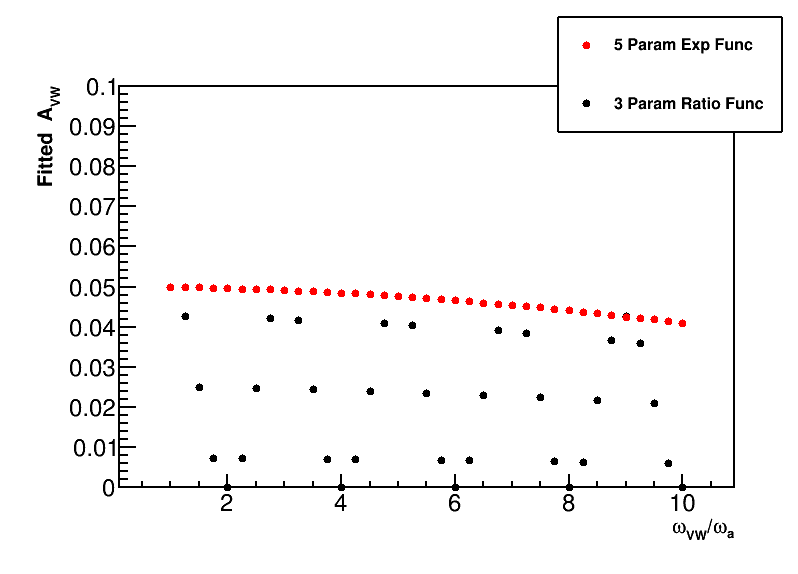
\includegraphics[width=.8\textwidth]{Fitted_Avw_Vs_Wvw_1x-10x}
%     \caption[]{Fitted VW amplitude in a Toy MC as a function of the VW frequency divided by the \gmtwo frequency. In red are the fitted amplitudes with a simple five parameter function, and in black are the fitted amplitudes with a three parameter ratio function. The input VW amplitude was 0.05, and the VW effect was constant throughout the Toy MC ``fill.'' There is a slight fall off of the red points due to the effects of the higher frequencies interacting with the bin width causing a reduction in the fitted amplitude; if an integral fit is used then this fall off is eliminated. What can be seen is that for even frequencies the VW effect dies away in the ratio fit, while for odd frequencies it does not.}
%     \label{fig:VW1x-10x}
% \end{figure}
% %  \texttt{/gm2/app/users/nkinnaird/RatioAnalysis/gm2Dev\_v9\_21\_03/srcs/gm2analyses/macros/RatioMacro/ToyMC/VW\_MC/OnlyVW/grid/ratioToyHists-OnlyVW-1x-10x-37iters.root}


% \begin{figure}[]
%     \centering
%     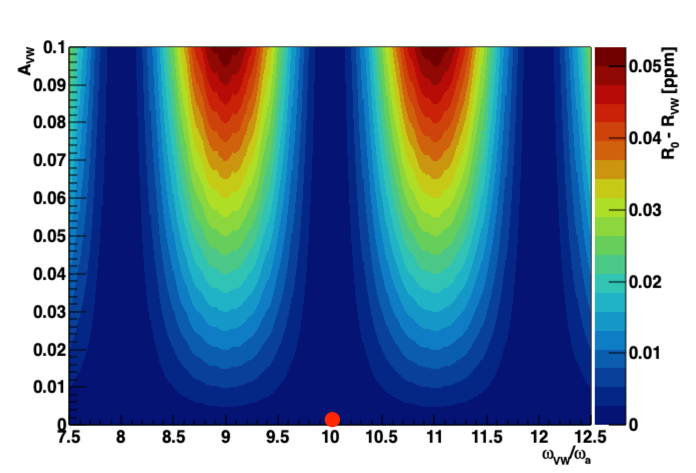
\includegraphics[width=.8\textwidth]{VWRatioDiff}
%     \caption[]{Plotted is the difference in the maximum value of the ratio with and without a VW function included, as a function of both the amplitude of the VW effect and the VW frequency in units of the \gmtwo frequency, in a toy Monte-Carlo simulation. Note that this is not $\boldsymbol{R}$ the frequency fit parameter, but the actual value of the ratio fit function. The difference reaches a minimum for even multiples of the \gmtwo frequency, where the VW effect divides out almost entirely. The $n = 0.108$ datasets, including the 60h and Endgame datasets, live at the bottom center of this plot, marked by a red circle, where the VW frequency is nearly equal to 10 times the \gmtwo frequency, and the difference in the ratio is approximately \SI{5e-6}{} at 30 $\mu s$. Plot courtesy of James Mott.}
%     \label{fig:VWRatioDiff}
% \end{figure}


\begin{figure}[]
\centering
    \begin{subfigure}[t]{0.7\textwidth}
        \centering
        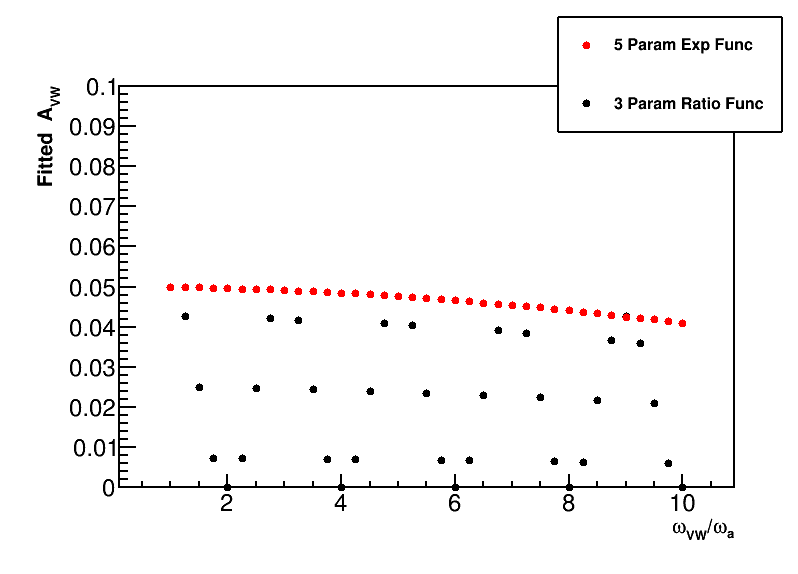
\includegraphics[width=\textwidth]{Fitted_Avw_Vs_Wvw_1x-10x} % \texttt{/gm2/app/users/nkinnaird/RatioAnalysis/gm2Dev\_v9\_21\_03/srcs/gm2analyses/macros/RatioMacro/ToyMC/VW\_MC/OnlyVW/grid/ratioToyHists-OnlyVW-1x-10x-37iters.root}
        \caption{Fitted VW amplitude with a five parameter function in red and a three parameter ratio function in black. The input amplitude was 0.05. The slight fall off of the red points is due to the high frequencies interacting with the bin widths; performing an integral fit removes this trend.}
    \end{subfigure}%

    \begin{subfigure}[t]{0.7\textwidth}
        \centering
        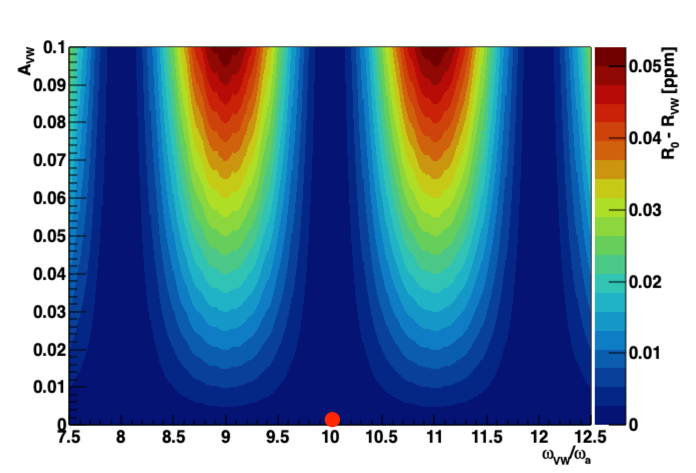
\includegraphics[width=\textwidth]{VWRatioDiff}
        \caption{The difference in the maximum value of the ratio (not the fit parameter \textbf{R}), as a function of VW frequency and amplitude.The difference in the ratio is approximately \SI{5e-6}{} at \mus{30}.}
    \end{subfigure}
\caption[]{Two separate Toy MC simulations showing the division of a VW effect as a function of it's frequency in units of \wa. For even multiple frequencies the effect dies away while for odd multiples it is preserved.}
\label{fig:ToyMCVW}
\end{figure}



\begin{figure}[]
\centering
    \begin{subfigure}[t]{0.7\textwidth}
        \centering
        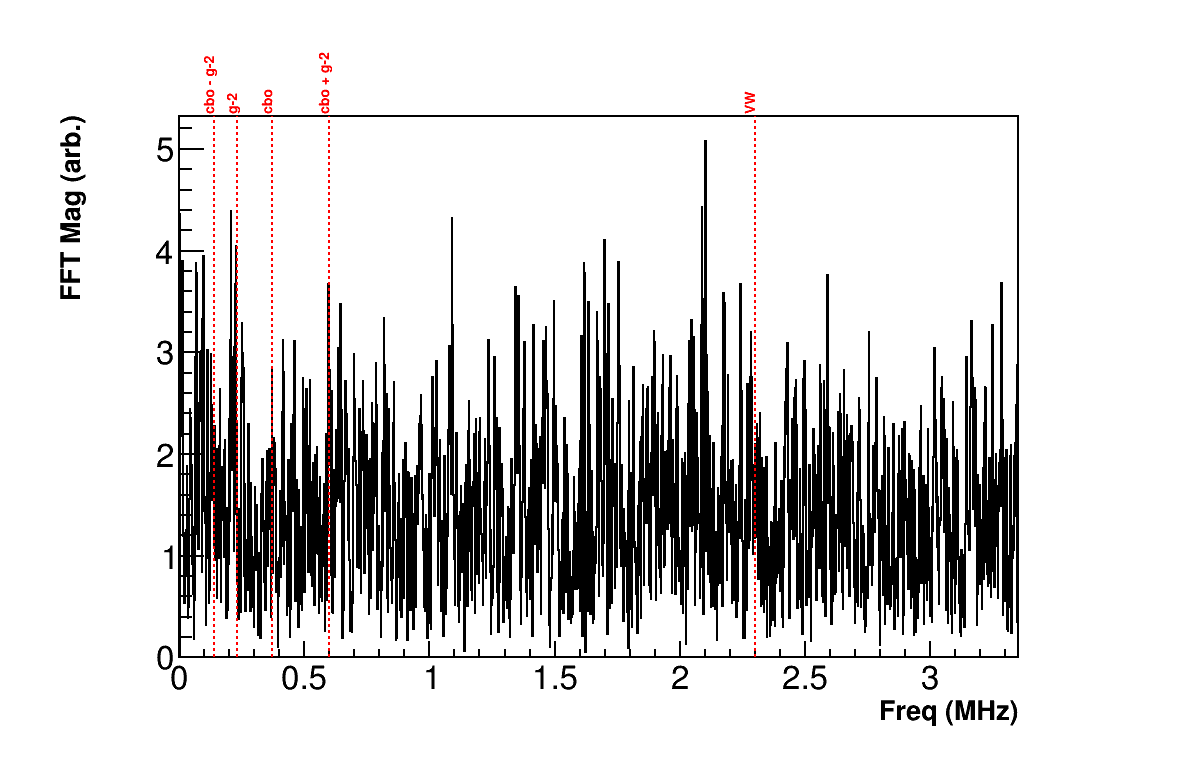
\includegraphics[width=\textwidth]{FFT_3param_allTimes} % From file \texttt{/gm2/data/users/nkinnaird/Ratio/60h-FinalProduction/RandSeeds/FitIterations/output-60h-FinalProduction-RandSeeds-1sttest.root} \texttt{FitPass0}.
        \caption{All times, \SIrange{30.2}{650}{\micro s}.}
    \end{subfigure}%

    \begin{subfigure}[t]{0.7\textwidth}
        \centering
        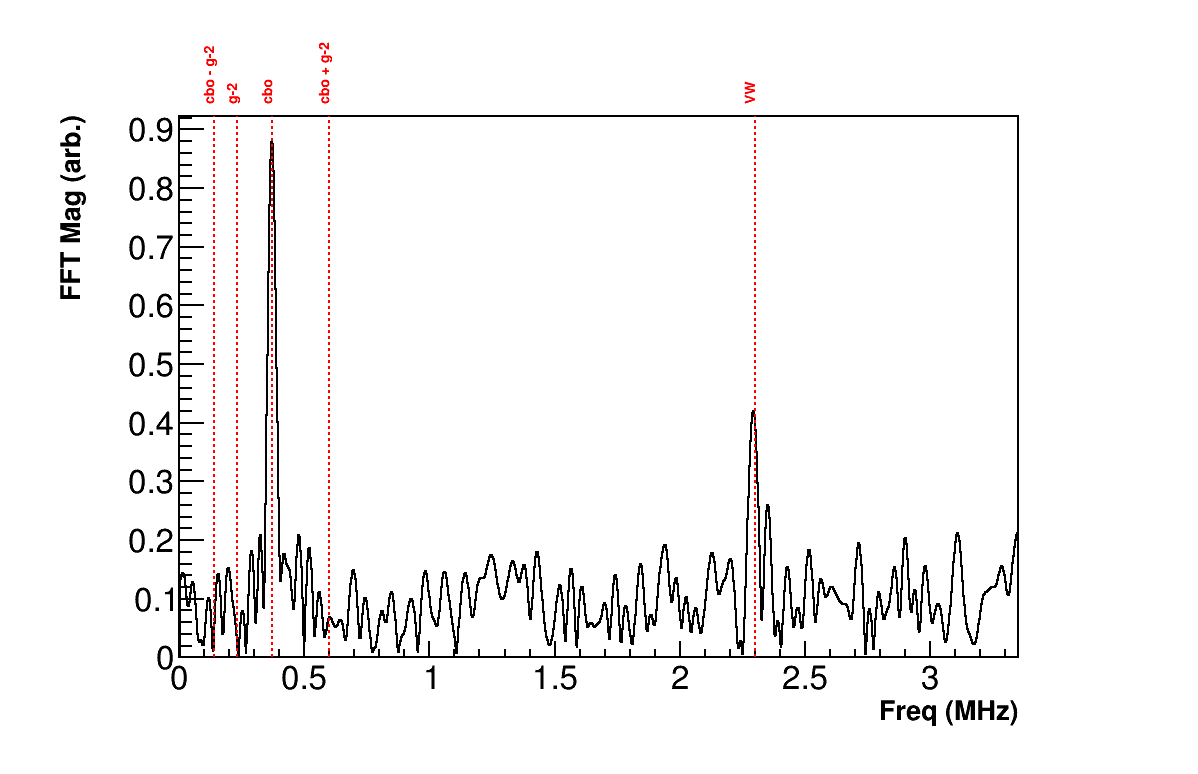
\includegraphics[width=\textwidth]{FFT_3param_earlyTimes} % From file \texttt{/gm2/data/users/nkinnaird/Ratio/60h-FinalProduction/RandSeeds/FitIterations/output-60h-FinalProduction-RandSeeds-1sttest.root} \texttt{FitPass0}.
        \caption{Early times, \SIrange{30.2}{60.2}{\micro s}.}
    \end{subfigure}
\caption[]{FFT of fit residuals using a 3 parameter ratio function to fit the 60h dataset. Peaks can be seen when looking at fit residuals over early times as opposed to all times. The size of the VW peak greatly depends on the choice of random seed. The CBO peak can also be seen.}
\label{fig:FFT_3param}
\end{figure}


\begin{figure}[]
    \centering
    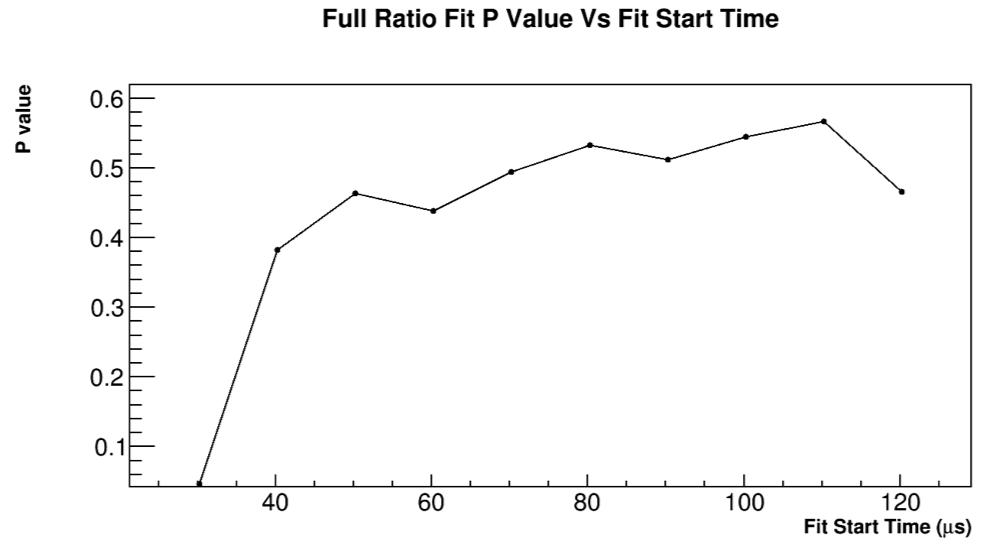
\includegraphics[width=.7\textwidth]{Pvalue_Endgame}
    \caption[]{P value vs fit start time for the Endgame dataset. A sharp rise can be seen at early times. A similar trend, though less severe, can be seen for the 60h dataset.}
    \label{fig:Pvalue_Endgame}
\end{figure}


\clearpage






The smallness of the VW signal in the ratio method analysis is the first of the problems in including it in the fit. First one might ask however whether it should be included in the fit at all. There are a couple of reasons why I think it should probably be included:
\begin{enumerate}
	\item\label{item:FFTpeak}{A peak in the FFT of the fit residuals can be seen.}
	\item\label{item:VWamp}{When the amplitude of the VW is allowed to float (with some or all of the others parameters fixed, whatever configuration is necessary to get a converging fit), then the VW amplitude converges to a non-zero value.}
	\item\label{item:pVal}{The p value of the fit improves when including the VW, on the order of 8\% for the 60h dataset, and on the order of 40\% for the Endgame dataset. This is reflected in a fit start scan of the p value, which shows a rise for the first \SIrange{20}{30}{\micro s} of the fit or so.}
	\item\label{item:Rchange}{The value of R changes on the order of \SIrange{30}{60}{ppb} depending on the dataset, which parameters are fixed, and what the random seed is.}
\end{enumerate}
It is the combination of items \ref{item:FFTpeak} and \ref{item:pVal} that I think are the real suggestions that I should be including the VW in the ratio fits. A couple of confusing things end up arising though, both around the idea that I should need to include the VW and what I see when I do so.


\section{60h and Endgame Datasets - An even multiple}

The 60h and Endgame datasets run at an n value of 0.108, which just so happens to put the VW frequency at nearly 10 times the \gmtwo frequency, specifically $\omega_{VW} \approx 10.04 \cdot \omega_{a}$ at $t = \infty$. (Remember that in these datasets the CBO frequency and by extension the VW frequency is changing over time, making this whole picture more complicated.) The ratio method, by definition, extracts out the \gmtwo frequency and by extension divides out frequencies which are an even multiple of the \gmtwo frequency. This can be seen in \figref{fig:VW1x-10x}, and the same is shown in a different way in \figref{fig:VWRatioDiff}. Because of this, I would expect for there to be no signal for the VW effect in the 60h and Endgame datasets. My only guess for why it still appears is that the VW frequency is changing over the course of a fill, so it still gets into the data in a way that can be seen. 








My plan would then be to include the VW in the ratio fit, with those VW parameters to which the ratio fit can't fit effectively, the frequency, lifetime, and sometimes phase, fixed from a T method fit, and the amplitude allowed to float. What then happens strangely enough however is that the VW amplitude in the ratio fit floats to unphysically high values, as seen in \figref{fig:ratioFit_highVWamp} where the amplitude is 0.2043 compared to the T method VW fitted amplitude in \figref{fig:TmethodFit_lowVWamp} at 0.003297, a factor of 62 increase. This factor difference varies wildly from seed to seed, but always remains very high. (Here it can be seen that the VW phase is floated in the fits and varies between the two, probably influencing the final fitted values.) If I include the VW and fix all parameters to the results from the T method fit, then what happens is R changes be nothing (less than 1 ppb) and the VW peak is unchanged. It seems the fit really does prefer such a high amplitude, which I still don't understand.


\begin{figure}[]
\centering
    \begin{subfigure}[]{0.6\textwidth}
        \centering
        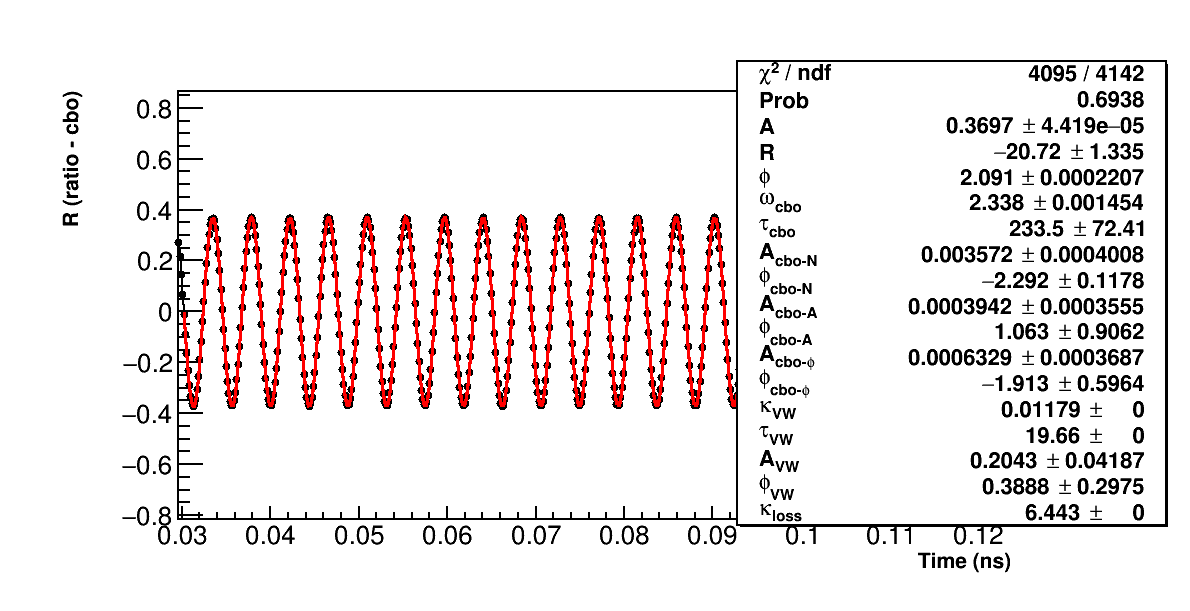
\includegraphics[width=\textwidth]{ratioFit_highVWamp}
        \caption{Ratio fit results with VW included of 60h dataset.}
    \label{fig:ratioFit_highVWamp}
    \end{subfigure}%
    \vspace{1cm}
    \begin{subfigure}[]{0.6\textwidth}
        \centering
        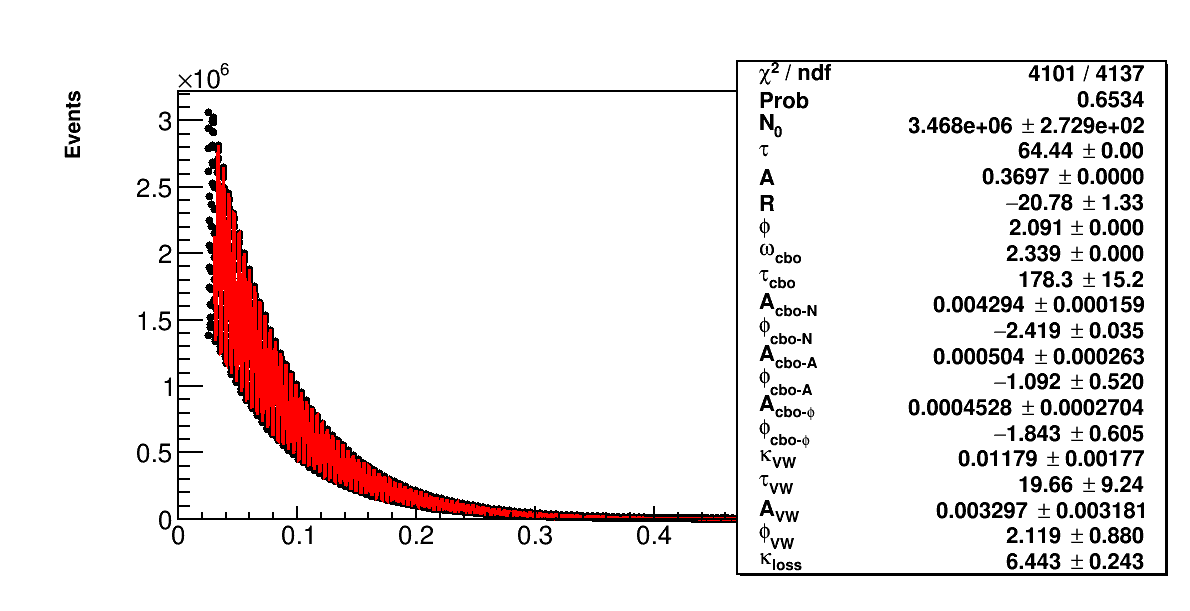
\includegraphics[width=\textwidth]{TmethodFit_lowVWamp}
        \caption{T method fit results of 60h dataset.}
    \label{fig:TmethodFit_lowVWamp}
    \end{subfigure}
\caption[]{}
\end{figure}
% \texttt{/gm2/data/users/nkinnaird/Ratio/60h-FinalProduction/RandSeeds/FitIterations/output-60h-FinalProduction-RandSeeds-1sttest.root} \texttt{FitPass0}

One thing I considered was whether the ratio method and fit really does somehow artificially raise the VW amplitude. Seems very unlikely but I made a Toy MC with a large VW effect and checked what came out, the first results of which are shown in \figref{fig:VW1x-10x}. That figure used the results from a 3 parameter ratio function, or 
    \begin{align} \label{eq:threeparamratio}
        R(t) \approx A \cos(\omega_{a}t),
    \end{align}
whereas I'm really fitting with the function
    \begin{gather}
        R(t) = \frac{2f(t) - f_{+}(t) - f_{-}(t)}{2f(t) + f_{+}(t) + f_{-}(t)}, \\
        f_{\pm}(t) = f(t \pm T_{a}/2), \\
        f(t) = V(t) \cdot (1 + A \cdot \cos(\omega_{a}t + \phi)),
    \label{eq:fullratiofunction}
    \end{gather}
or as I call it the full ratio function, with $V(t)$ being the VW effect, and without other background terms which are unnecessary in the Toy MC. Fitting with this function yields the results shown in \figref{fig:FittedAVW_FullRatioFunc}. As shown, the fitted VW amplitude dies away at even frequencies for the 3 parameter ratio function, however there is some interesting behaviour with the results from the full ratio function. The results do in fact make perfect sense when considering Equation~\ref{eq:fullratiofunction} more carefully. What $f(t)$ represents in that function is the five parameter function, barring the $N_{0}$ and $\tau_{\mu}$ terms which divide out. In that case the fitted amplitude between the five paramter function and the T method function should be the exact same. This is the case between the red and blue points until the frequency gets very close to 10 times \wa. As seen the fit becomes unstable, with largely differing amplitudes in some cases with large error bars. There are also some points with values different from the real value, and with small, inconsistent errors. What is happening here makes sense in that the VW effect in the ratio has almost completely divided out, but yet I am trying to fit it with a function where the value of $A_{VW}$ does not particularly matter. In essence I believe I am using a term in the fit function which isn't particularly well motivated. 


\begin{figure}[]
\centering
    \begin{subfigure}[]{0.46\textwidth}
        \centering
        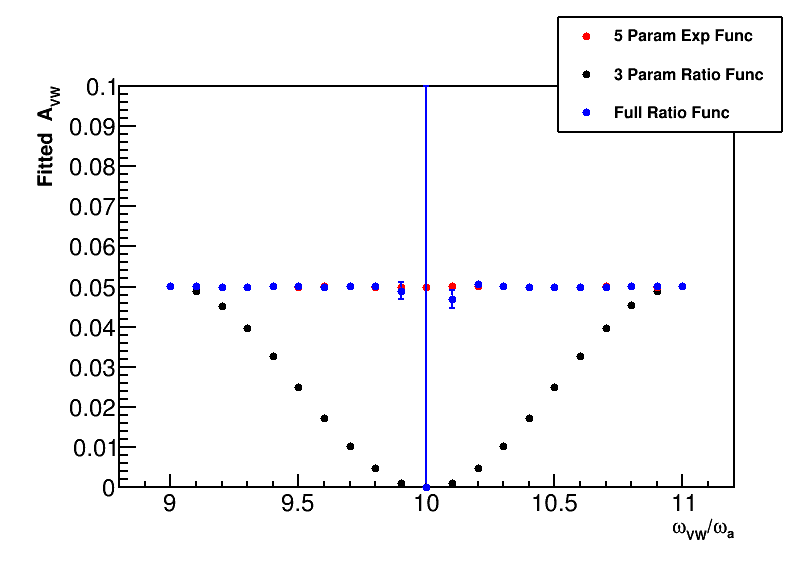
\includegraphics[width=\textwidth]{Fitted_Avw_Vs_Wvw-9x-10x}
        \caption{$9\times$ to $11\times$ \wa.}
    \end{subfigure}% %you need this % here to add spacing between subfigures
    \hspace{1cm}
    \begin{subfigure}[]{0.46\textwidth}
        \centering
        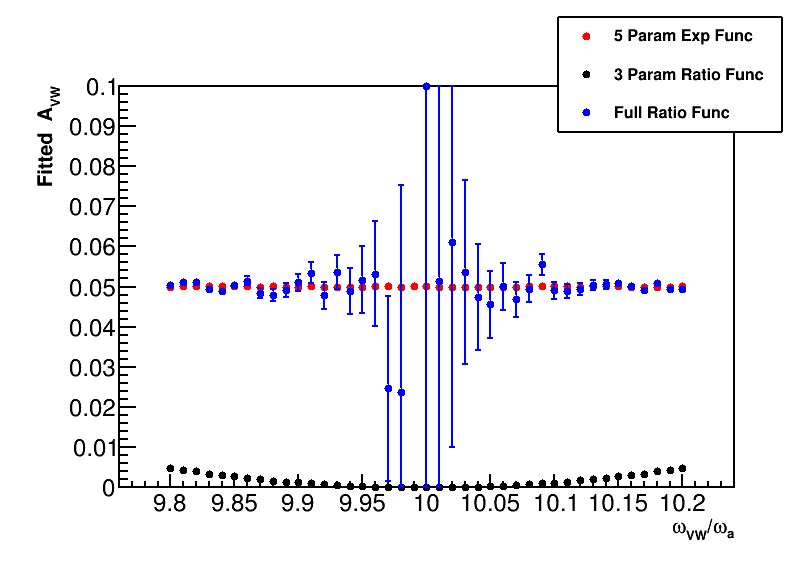
\includegraphics[width=\textwidth]{Fitted_Avw_Vs_Wvw-10x}
        \caption{$9.8\times$ to $10.2\times$ \wa.}
    \end{subfigure}
\caption[]{Fitted VW amplitude as a function of frequency and with different types of fit functions. }
\label{fig:FittedAVW_FullRatioFunc}
\end{figure}
% \texttt{/gm2/app/users/nkinnaird/RatioAnalysis/gm2Dev\_v9\_21\_03/srcs/gm2analyses/macros/RatioMacro/ToyMC/VW\_MC/OnlyVW/grid/ratioStyleFunc}


If my fit results to the real data returned values with large error bars consistent with 0, or consistent with the T method results, then I believe there wouldn't be a problem, and I could do one or the other. Conceptually, I think the `right' answer would be that the T method values are right, and I should just fix the values in the ratio method to them and call it a day. However, going back up to a point in an earlier paragraph, this doesn't improve the fit and the VW signal still appears in the data unchanged. So at the end of the day I have this problem, which seems contradictory in that I don't think I should be able to see the VW but can, and that my fit shouldn't prefer a specific amplitude but does, and that amplitude is an unphyisically large value. 


I was going to leave it out in the 60h dataset and call it a day, until the Endgame results showed a much larger change in the p value that seems un-ignorable.


Probably show said change or picture here or something - look up these results again






\section{9d Dataset - a different problem}


While in the 60h and Endgame datasets the VW frequency is nearly 10 times \wa, in the 9d the frequency is closer to an odd multiple, or $\omega_{VW} \approx 8.87 \cdot \omega_{a}$ at $t = \infty$. With what I've shown so far, I expect the VW signal to be easily fittable with an amplitude equal to that from the T method results. Looking at per calo fit results in \figref{fig:9d-PerCalo-VW}, the VW phases and amplitudes are consistent between the T method and ratio method results. As shown there are no observable differences. When I look at the fits to the sum of the calorimeter data however, I see a systematically smaller VW amplitude in the ratio fit results as compared to the T method results. This is true for all random seeds as shown in \figref{fig:vw-fixed-w-tau-9d-randseeds}. While I expect a reduction in the VW amplitude from per calo fits to the calorimeter sum fit, as the phases go from 0-2$\pi$ around the ring, I still expect the amplitudes to be consistent between the T method and ratio method. If I take calorimeters adjacent to each other around the ring versus calorimeters separated from each other, then I see the behaviour. So what seems to be happening is that there is a cancellation when adding the calorimeters together in the ratio method that doesn't occur in the T method. That is something I don't understand, and can't come up with a reason why that should happen. I'm not sure if this is at all related to the previously discussed problem or not, whether it's another symptom or something else strange. 



\begin{figure}[]
\centering
    \begin{subfigure}[]{0.46\textwidth}
        \centering
        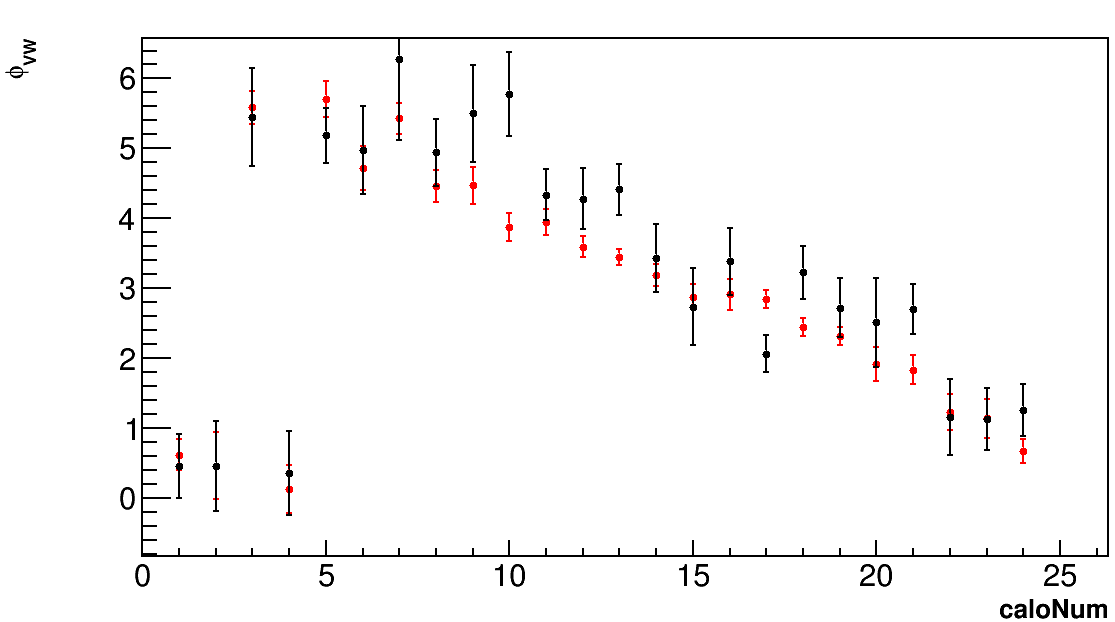
\includegraphics[width=\textwidth]{9d-CaloFits-VW-Phases}
        \caption{VW phases per calo in the 9d dataset.}
    \end{subfigure}% %you need this % here to add spacing between subfigures
    \begin{subfigure}[]{0.46\textwidth}
        \centering
        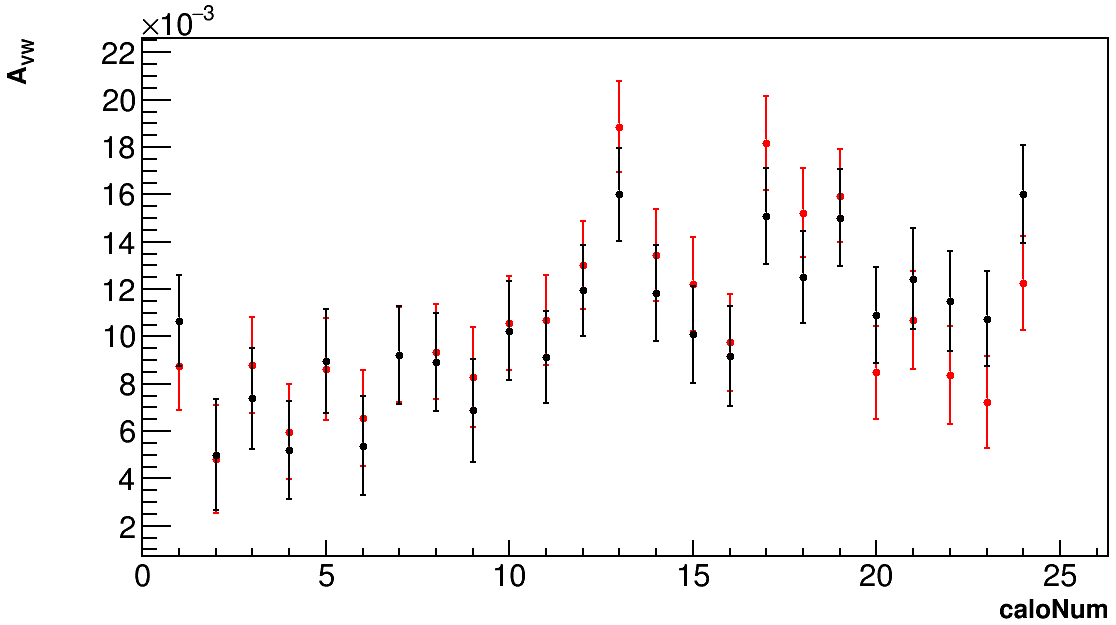
\includegraphics[width=\textwidth]{9d-CaloFits-VW-Amps}
        \caption{VW amplitudes per calo in the 9d dataset.}
    \end{subfigure}
\caption[]{Red points are T method results and black points are ratio method results. In the ratio fits, the VW frequencies and lifetimes are fixed to those from the T method results.}
\label{fig:9d-PerCalo-VW}
\end{figure}
% \texttt{/gm2/data/users/nkinnaird/Ratio/9d-FinalProduction/SingleIteration/temptests/CaloFits-VW-w-tau-fixed}

\begin{figure}[]
    \centering
    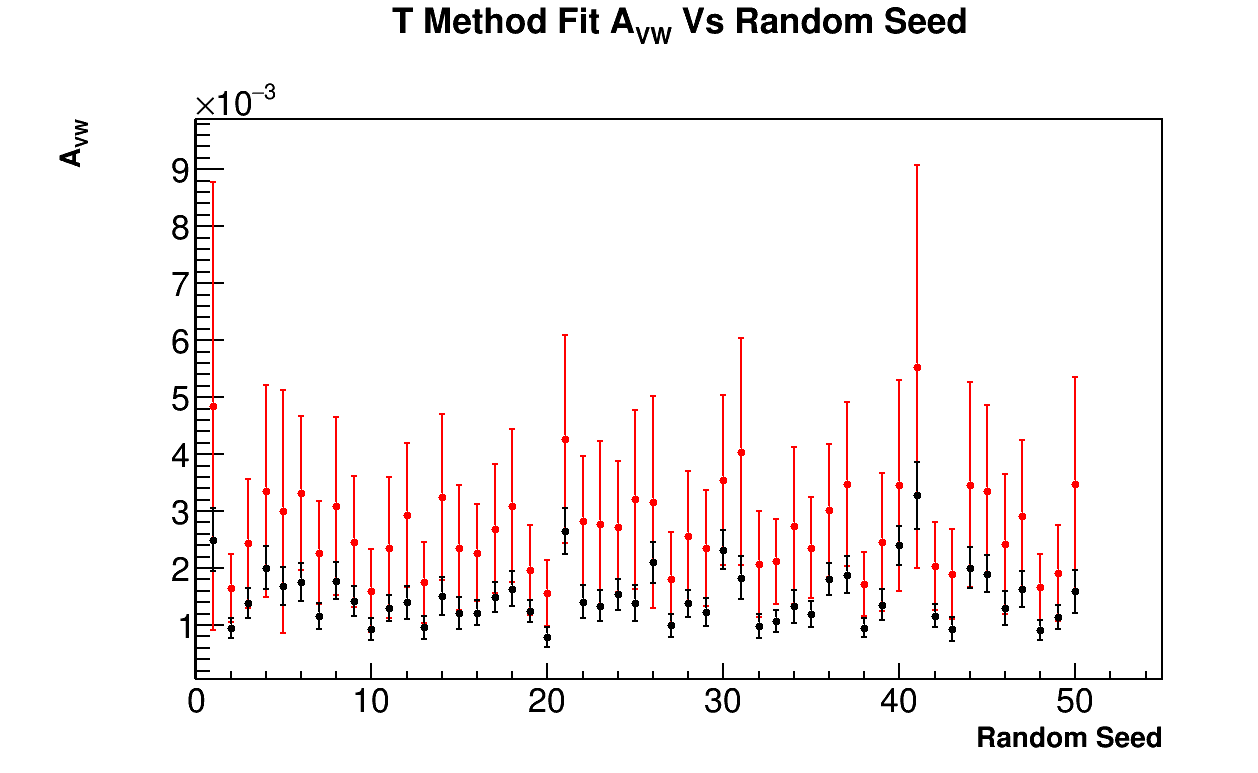
\includegraphics[width=0.7\textwidth]{vw-fixed-w-tau-9d-randseeds}
    \caption[]{VW amplitudes as a function of random seed for T method fits compared to ratio method fits. T method fits are in red and ratio fits are in black. The error bars are smaller on the ratio fits because the VW frequencies and lifetimes are fixed to those from the T method fits. There is a consistently smaller VW amplitude in the ratio fits as compared to the T method fits.}
    \label{fig:vw-fixed-w-tau-9d-randseeds}
\end{figure}
% \texttt{/gm2/data/users/nkinnaird/Ratio/9d-FinalProduction/RandomSeeds/tests\_with\_VW/fixed-vw-w-tau}


\section{Correlations and fit start scans}




\section{Randomizing out the effect...}

\cite{wa_presentation}



\printbibliography



% \begin{figure}[]
%     \centering
%     \includegraphics[width=\textwidth]{}
%     \caption[]{}
%     \label{fig:}
% \end{figure}


% \begin{figure}[]
% \centering
%     \begin{subfigure}[t]{0.7\textwidth}
%         \centering
%         \includegraphics[width=\textwidth]{}
%         \caption{}
%     \end{subfigure}%

%     \begin{subfigure}[t]{0.7\textwidth}
%         \centering
%         \includegraphics[width=\textwidth]{}
%         \caption{}
%     \end{subfigure}
% \caption[]{}
% \label{}
% \end{figure}


\end{document}

